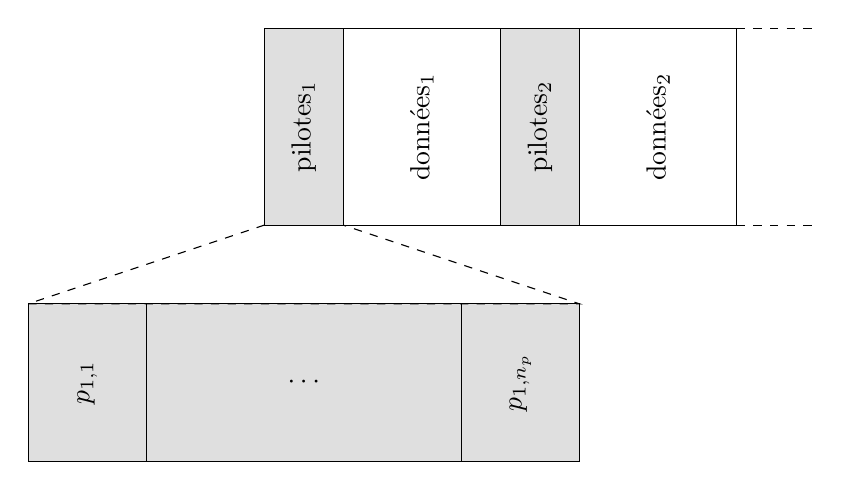
\begin{tikzpicture}[scale = 2]
    \draw[fill = lightgray!50!white](0,0) rectangle (0.5,1.25) node[midway, rotate = 90]
    {\Orange{pilotes}$\bm{_1}$};
    
    \draw(0.5,0) rectangle (1.5,1.25)node[midway, rotate = 90]
    {\Blue{données}$\bm{_1}$};
    
    \draw[fill = lightgray!50!white](1.5,0) rectangle (2,1.25) node[midway, rotate = 90]
    {\Orange{pilotes}$\bm{_2}$};
    
    \draw(2,0) rectangle (3,1.25)node[midway, rotate = 90]
    {\Blue{données}$\bm{_2}$};
    
    \draw[dashed] (3,0) --++ (0.5,0);
    \draw[dashed] (3,1.25) --++ (0.5,0);

    \draw [fill = lightgray!50!white](-1.5,-1.5) rectangle(2,-0.5) node[midway]
    {$\cdots$};
    
    \draw [fill = lightgray!50!white] (-1.5,-1.5) rectangle(-0.75,-0.5) 
    node[midway, rotate = 90]{$\Orange{p}_{\bm{1},1}$};
    
    \draw [fill = lightgray!50!white] (1.25,-1.5) rectangle(2,-0.5) 
    node[midway, rotate = 90]{$\Orange{p}_{\bm{1},n_p}$};

    \draw[dashed] (0,0) -- (-1.5,-0.5) --++ (3.5,0) -- (0.5,0);
    \draw (0,-1.5) node{};
\end{tikzpicture}

